%!TEX root = main.tex
\def\macrofilledtile{
\draw [fill=lightgray,opacity=0.99]  (\x + 0, \y) rectangle (\x+1,\y+1);
}
\def\macropositivetile{
     \def\south{}
     \def\east{}
     \def\north{}
     \def\west{} 
     \draw (\x + 0, \y) --  (\x+1,\y) node [pos=0.5,above] {\south} -- (\x+1,\y+1) node [pos=0.5,left] {\east} -- (\x+0,\y+1) node [pos=0.5,above] {\north} --  (\x + 0, \y)  node [pos=0.5,left] {\west};
}
\def\macronegativetile{
     \def\south{}
     \def\east{}
     \def\north{}
     \def\west{} 
     \draw (\x + 0, \y) --  (\x+1,\y) node [pos=0.5,above] {\south} -- (\x+1,\y+1) node [pos=0.5,left] {\east} -- (\x+0,\y+1) node [pos=0.5,above] {\north} --  (\x + 0, \y)  node [pos=0.5,left] {\west};
}
\def\matchingcolor{2pt}
% begin snake graph 1011101100 or 2,3,1,2,3 with matching generated by d and k
 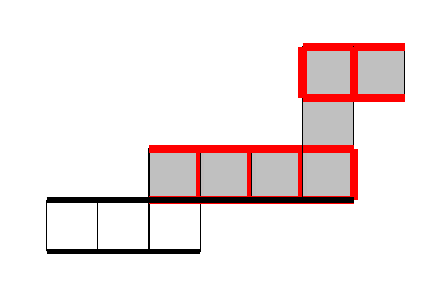
\begin{tikzpicture}[scale=0.65,font=\scriptsize]
 \foreach \x in {0,1,...,2} % bottom row 
 {
%     \draw (\x + 0, 0) -- (\x+1,0) -- (\x+1,1)-- (\x+0,1) -- cycle;
\def\y{0}
     \ifthenelse{\x = 0 \OR \x =2}
     {
     \macropositivetile
     }{
     \macronegativetile
     }
     \ifthenelse{\x = 0 \OR \x =2}{\draw[line width=\matchingcolor] (\x + 0, \y+0) -- (\x+1,\y+0);}{} % south
     \ifthenelse{\x = 0}{\draw[line width=\matchingcolor] (\x + \y+0, \y+1) -- (\x+1,\y+1);}{} % north
 }
\def\y{1}
 \foreach \x in {2,...,5} % second from bottom row
 {
     \ifthenelse{\x = 2 \OR \x = 3}{\macrofilledtile}{}
     %\ifthenelse{\x = 2}{\draw (\x + 0.5, \y+0.5) node {\boxed{$d$}}; }{}
     %\ifthenelse{\x = 3}{\draw (\x + 0.5, \y+0.5) node {{$e$}}; }{}
     %\draw (\x + 0, \y) -- (\x+1,\y) -- (\x+1,\y+1)-- (\x+0,\y+1) -- cycle;
     \ifthenelse{\x = 3 \OR \x =5}{\macropositivetile}{\macronegativetile}
     %\ifthenelse{\x = 2}{\draw[line width=\matchingcolor] (\x+0, \y+0) -- (\x, \y+1);}{} % west
     \ifthenelse{\x = 2}{\draw[red, %densely dashed, 
     line width=1.5*\matchingcolor] (\x+0, \y+0) -- (\x+1, \y+0);}{} % south
     \ifthenelse{\x = 2}{\draw[red, %densely dashed, 
     line width=1.5*\matchingcolor] (\x+0, \y+1) -- (\x+1,\y+1);}{} % north
      \ifthenelse{\x = 3}{\draw[red, %densely dashed,
      line width=1.5*\matchingcolor] (\x+1, \y) -- (\x+1,\y+1);}{} % east
      %\ifthenelse{\x = 3}{\draw[line width=\matchingcolor] (\x+0, \y+0) -- (\x+1, \y+0);}{} % south
     %\ifthenelse{\x = 3}{\draw[line width=\matchingcolor] (\x+0, \y+1) -- (\x+1,\y+1);}{} % north
      \ifthenelse{\x =5}{\draw[line width=\matchingcolor] (\x+0, \y+0) -- (\x+1, \y+0);}{} % south
 } 
\def\y{2}
 \foreach \x in {5} % third from bottom row
 {
     \macrofilledtile
     %\draw (\x + 0, \y) -- (\x+1,\y) -- (\x+1,\y+1)-- (\x+0,\y+1) -- cycle;
     \macronegativetile
     %\ifthenelse{\x = 5}{\draw[line width=\matchingcolor] (\x+0, \y+0) -- (\x, \y+1);}{} % west
     %\ifthenelse{\x = 5}{\draw[line width=\matchingcolor] (\x+1, \y) -- (\x+1,\y+1);}{} % east
     \ifthenelse{\x = 5}{\draw[red,%densely dashed,
     line width=1.5*\matchingcolor] (\x+0, \y+0) -- (\x+1, \y+0);}{} % south
     %\draw (\x + 0.5, \y+0.5) node {{$h$}};
 }  
\def\y{3}
\foreach \x in {5,6} % fourth from bottom row
{
    \macrofilledtile
     %\draw (\x + 0, \y) -- (\x+1,\y) -- (\x+1,\y+1)-- (\x+0,\y+1) -- cycle;
     \ifthenelse{\x = 5}
     {\macropositivetile}{\macronegativetile}
     %\ifthenelse{\x = 5}{\draw[line width=\matchingcolor] (\x+0, \y+1) -- (\x+1,\y+1);}{} % north
     \ifthenelse{\x = 5}{\draw[red,%densely dashed,
     line width=1.5*\matchingcolor] (\x+0, \y+0) -- (\x, \y+1);}{} % west

     %\ifthenelse{\x = 6}{\draw[line width=\matchingcolor] (\x+1, \y) -- (\x+1,\y+1);}{} % east
     \ifthenelse{\x = 6}{\draw[red,%densely dashed,
     line width=1.5*\matchingcolor] (\x+0, \y+0) -- (\x+1, \y+0);}{} % south
     \ifthenelse{\x = 6}{\draw[red,%densely dashed,
     line width=1.5*\matchingcolor] (\x+0, \y+1) -- (\x+1,\y+1);}{} % north
     %\ifthenelse{\x = 5}{\draw (\x + 0.5, \y+0.5) node {{$i$}}; }{}
     %\ifthenelse{\x = 6}{\draw (\x + 0.5, \y+0.5) node {\boxed{$j$}}; }{}
 } 
\end{tikzpicture} % end of matching subword with 1 missing